\section{Marktformen}
\textbf{Maximaler Gewinn:}
\settowidth{\MyLenA}{Vollkommene Konkurrenz~~}
\begin{tabular}{@{}p{\the\MyLenA}%
 				@{}p{\linewidth-\the\MyLenA}}
 	Vollkommene Konkurrenz & Preis = Grenzkosten\\
	Monopolist & Grenzerlös = Grenzkosten
\end{tabular}

\begin{description}\itemsep0em
	\item [Grenzerlös] Erlös für eine zusätzliche verkaufte Einheit
	\item [Cournotscher Punkt] Schnittpunkt der Grenzerlös- mit der Grenzkostenkurve
\end{description}

\begin{center}
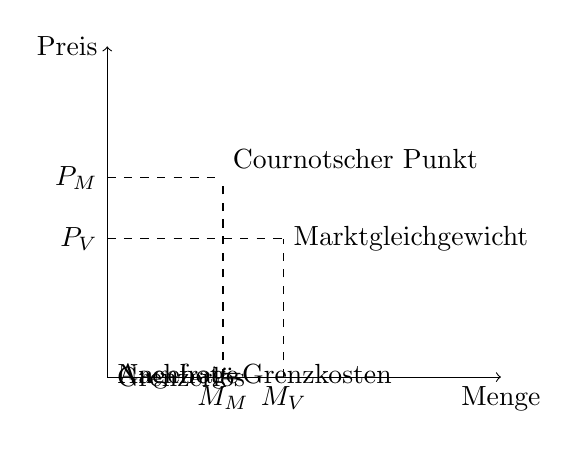
\begin{tikzpicture}
    %\draw[very thin,color=gray] (-0.1,-1.1) grid (3.9,3.9);
    \draw[->] (0,0) -- (5,0) node[below] {Menge};
    \draw[->] (0,0) -- (0,4.2) node[left] {Preis};
    \draw[thick, domain=0.25:3.8] plot[id=n] function{-x + 4} node[right] {Nachfrage};
    \draw [thick, domain=0.25:2.8] plot[id=a] function{x * x/4 + 0.5}  node[right] {Angebot=Grenzkosten};
    \draw [dotted, domain=0.25:1.8] plot[id=z] function{-2 * x + 4} node[right] {Grenzerlös};
	% monopol
	\draw [dashed] (1.47, 0)  node [below] {$M_M$} -- (1.47, 2.53) node[above right] {Cournotscher Punkt};
	\draw [dashed](0,2.53) node [left] {$P_M$} -- (1.47,2.53);
	% vollkommene Konkurrenz
	\draw [dashed](2.243,0) node [below] {$M_V$} -- (2.243,1.757) node[right] {Marktgleichgewicht};
	\draw [dashed](0,1.757) node [left] {$P_V$}-- (2.243,1.757);
\end{tikzpicture}
\end{center}

Der Monopolist setzt die Menge $M_M$ zum Preis $P_M$ ab.\\ 
Bei vollkommener Konkurrenz wird die grössere Menge $M_V$ zum geringeren Preis $P_V$ abgesetzt.

\begin{tabular}{l|p{1.6cm}|p{1.6cm}|p{1.6cm}}
	& \multicolumn{3}{c}{Anbieter}\\
	Nachfrager & \multicolumn{1}{c|}{Viele} & \multicolumn{1}{c|}{Wenige} & \multicolumn{1}{c}{Einer}\\\hline
	Viele & Polypol & Angebots-oligopol & Angebots-monopol \\\hline
	Wenige & Nachfrage-oligopol & Zweiseitiges (bilaterales) Oligopol & Angebots-monopol \& Nachfrage- oligopol\\\hline
	Einer & Nachfrage-monopol & Nachfrage-monopol \& Angebots-oligopol & Zweiseitiges (bilaterales) Monopol \\\hline
\end{tabular}

\subsection{Monopolistische Konkurrenz}
Markenprodukte (Coca Cola) sind typisch dafür. Monopol bezüglich Marke, Oligopol bezüglich Substituten.
Dies führt zu einem geringen Spielraum bei den Preisen.

Der übliche Entwicklung ist:
\begin{enumerate}\itemsep0em
	\item Monopol, wenn ein neues Produkt erfunden wird (z.\,B. iPad)
	\item Monopolistische Konkurrenz, viele Anbieter bieten ähnliches (z.\,B. Android Tablets)
	\item Oligopol, sobald wenige überlebt haben
\end{enumerate}
